\documentclass[fr]{../../../../../../epltest}


\hypertitle{Compléments d'électricité (partie dispositifs)}{5}{ELEC}{1330}{2017}{Novembre}
{Maxime Wattiaux}
{Denis Flandre}
	
	\begin{center}
		\underline{PARTIE EXERCICE}
	\end{center}
	
	On considère la jonction NP en silicium représentée sur la figure 1 ci-dessous. La zone P ainsi que la zone de déplétion sont protégées de toute illumination par un cache. La zone N n'est par contre pas couverte et soumise à une génération constante G. La structure est suffisamment fine ($h \approx 0$) de sorte que les termes de génération peuvent être considérés constants dans le volume de la zone N. La zone de déplétion est supposée équitablement répartie entre les deux zones N et P, et est de longueur $d$ donnée. On supposera que la génération/recombinaison dans cette zone est constante et donnée par le facteur $U_0$. Une différence de potentiel $V$ est appliquées aux bornes de la diode (entre $x = - x_n$ et $x= x_p$) via des contacts ohmiques. On suppose $N_A$ et $N_D$ connus ainsi que $D_n$, $D_p$, $\tau_n$, $\tau_p$, $T$, $V$, $G$ et $U_0$. \\
	
	On supposera également que $x_p$ << $L_n$ et $x_n$ >> $L_p$.
	
	\begin{figure}[h!]
		\centering
		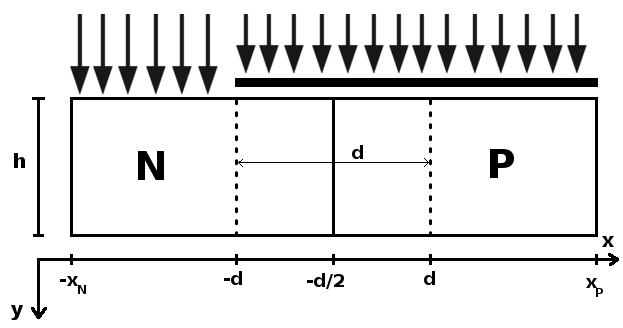
\includegraphics[scale=0.5]{pictures/interro.png}
		\caption{Jonction NP}
		\label{Jonction NP}
	\end{figure}
	
	On vous demande de trouver l'équation de la densité de courant $J$ dans la diode. \\
	
	Énoncez et justifiez clairement toutes les hypothèses simplificatrices que vous utilisez au cours de votre développement. \\
	
	\begin{enumerate}
		\item Déterminez les expressions générales des concentrations en porteurs minoritaires et de la densité de courant dans les deux zones quasi-neutres de la diode à partir des équations de transport.
		\item Donnez les conditions limites nécessaires au calcul de la densité de courant, pour chaque zone et chaque densité de courant en porteurs minoritaires. 
		\item Donnez l'expression de la densité de courant dans la diode en fonction des densités de courant dans chaque zone de la diode et éventuellement des termes de génération/recombinaison.
		\item En développant l'expression obtenue au point précédent, donnez l'expression finale du courant selon les paramètres connus du dispositif.
	\end{enumerate}
	
	Aide - La solution à une équation différentielle du type :
	
	\begin{equation*}
		\frac{\partial f}{\partial x^2} -kf = 0 \hspace{1cm} \text{est donnée par :} \hspace{1cm} f(x) = Ae^{\sqrt{k}x} + Be^{-\sqrt{k}x}
	\end{equation*}
	
	Décrivez qualitativement mais le plus précisément possible : 
	
	\begin{enumerate}
		\setcounter{enumi}{4}
		\item Que se passerait-il si le temps de vie des électrons augmente ? Discutez l'influence de ce paramètre sur vos hypothèses de calcul ainsi que sur l'intensité du courant total.
	\end{enumerate}
	
	\bigskip
	
	\textbf{REMARQUE :} Le formulaire de la partie dispositifs était fourni.
	
	\newpage
	
	\begin{center}
		\underline{PARTIE THÉORIE}
	\end{center}
	
	$\bullet$ Utilisez des schémas, formules, outils et concepts de base... et limitez le <<bla-bla>> au strict nécessaire.
	
	\begin{enumerate}
		\item Tracez dans un graphe (en échelle linéaire) et expliquez la courbe caractéristique courant-tension de la diode telle que vue dans le cours. Situez les différents régimes de fonctionnement de manière précise. Indiquez des valeurs numériques typiques.
		\item Détaillez l'équation $I-V$ correspondante au niveau physique et ses limites de validité. Définissez les paramètres technologiques et physiques qui influencent le courant.
		\item Discutez les hypothèses sous-jacentes et écarts entre théorie simple et mesures. Représentez les effets non-idéaux sur graphe $log(I)-V$
	\end{enumerate}
	
	
\end{document}